\subsection{Recordar contraseña}

  \paragraph{}En el caso de que dispongamos de un usuario válido para acceder a
  la aplicación pero hemos olvidado la contraseña, es posible generar una nueva,
  que será enviada al correo electrónico del usuario.

  \paragraph{}Para ello, en la pantalla inicial debemos pulsar el enlace
  \textit{Recordar contraseña}, que se encuentra a la derecha del botón
  \textit{OK} \ref{capturaBotonOK}. La imagen \ref{capturaRecordarPassword}
  muestra el enlace mencionado.

  \begin{figure}[!ht]
    \begin{center}
      \fbox{
      
\includegraphics[]{4.Funcionamiento_Aplicacion/4.2.Acceso_Sistema/4.2.1.Recordar_Password/Capturas/recordar_password.png}
      }
      \caption{Captura de pantalla del enlace \textit{Recordar contraseña}.}
      \label{capturaRecordarPassword}
    \end{center}
  \end{figure}

  \paragraph{}Una vez pulsado, la aplicación pedirá el correo electrónico del
  usuario para el cual se desea recuperar la contraseña de acceso, como se puede
  ver en la imagen \ref{capturaPedirCorreo}.

  \begin{figure}[!ht]
    \begin{center}
      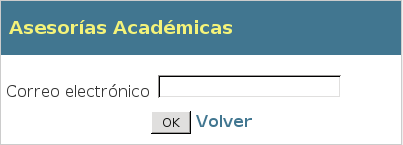
\includegraphics[]{4.Funcionamiento_Aplicacion/4.2.Acceso_Sistema/4.2.1.Recordar_Password/Capturas/pedir_correo.png}
      \caption{Captura de pantalla de la petición del correo electrónico para recuperar la contraseña.}
      \label{capturaPedirCorreo}
    \end{center}
  \end{figure}

  \paragraph{}Siempre es posible volver a la pantalla inicial pulsando el enlace
  \textit{Volver}, mostrado en la imagen \ref{capturaEnlaceVolver}.

  \begin{figure}[!ht]
    \begin{center}
      \fbox{
      
\includegraphics[]{4.Funcionamiento_Aplicacion/4.2.Acceso_Sistema/4.2.1.Recordar_Password/Capturas/enlace_volver.png}
      }
      \caption{Captura de pantalla del enlace \textit{Volver}.}
      \label{capturaEnlaceVolver}
    \end{center}
  \end{figure}

  \paragraph{}Si introducimos un correo electrónico válido, que esté asociado a
  un usuario de la base de datos de la aplicación, y pulsamos el botón
  \textit{OK} \ref{capturaBotonOK}, aparecerá un mensaje diciendo que la nueva
  contraseña se ha generado con éxito, la cual habrá sido enviada al correo
  electrónico introducido. Se puede ver una captura de pantalla de este mensaje
  en la imagen \ref{capturaPedirCorreoExito}.

  \begin{figure}[!ht]
    \begin{center}
      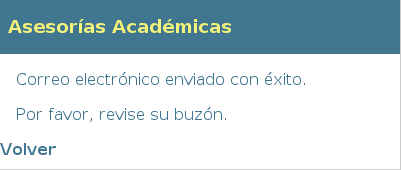
\includegraphics[]{4.Funcionamiento_Aplicacion/4.2.Acceso_Sistema/4.2.1.Recordar_Password/Capturas/pedir_correo_exito.png}
      \caption{Captura de pantalla del mensaje con éxito al recuperar la contraseña.}
      \label{capturaPedirCorreoExito}
    \end{center}
  \end{figure}

  \paragraph{}Pulsando en el enlace \textit{Volver}, mostrado en la imagen
  \ref{capturaEnlaceVolver}, volveremos a la pantalla inicial.

  \paragraph{}Si por el contrario introducimos un correo electrónico no válido,
  aparecerá un mensaje indicando tal circunstancia. La imagen
  \ref{capturaPedirCorreoInvalido} muestra tal mensaje.

  \begin{figure}[!ht]
    \begin{center}
      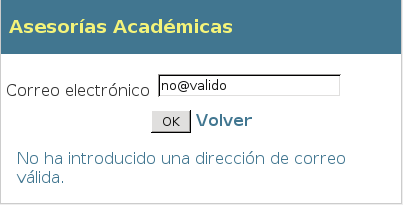
\includegraphics[]{4.Funcionamiento_Aplicacion/4.2.Acceso_Sistema/4.2.1.Recordar_Password/Capturas/pedir_correo_invalido.png}
      \caption{Captura de pantalla del mensaje no válido al recuperar la contraseña.}
      \label{capturaPedirCorreoInvalido}
    \end{center}
  \end{figure}

  \paragraph{}En última instancia, si el correo electrónico introducido es un
  correo electrónico válido, pero no pertenece a ningún usuario del sistema,
  también será indicado a través de un mensaje, como muestra la figura
  \ref{capturaPedirCorreoNoExito}.

  \begin{figure}[!ht]
    \begin{center}
      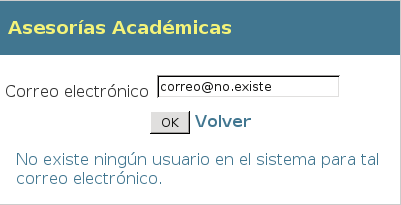
\includegraphics[]{4.Funcionamiento_Aplicacion/4.2.Acceso_Sistema/4.2.1.Recordar_Password/Capturas/pedir_correo_noexito.png}
      \caption{Captura de pantalla del mensaje sin éxito al recuperar la contraseña.}
      \label{capturaPedirCorreoNoExito}
    \end{center}
  \end{figure}
